\documentclass[a4paper, twoside, 11pt]{article}
% It is needed to use this command for automatic compilation in VSCode
% !TEX program = lualatexmk

%DOCUMENT, PREAMBLE AND MACROS DESIGNED FOR LuaLaTeX%
\newcommand{\fbar}{\FloatBarrier}

\usepackage{amsmath} %matematic package%
\usepackage{textcomp} %for miscellaneous symbols%
%\usepackage{times} %times font%
\usepackage{graphicx} %enhanced support for craphics%
%\usepackage{mathptmx} %use Times as default text font, and provide maths support%
\usepackage{cmap} %mapování znaků - vyhledávání v pdf%
\usepackage[czech]{babel}%CZ%
\usepackage[utf8]{inputenc}%kódování%
\usepackage[T1]{fontenc}%kódování%
\usepackage{multirow}%Multirow table support
\usepackage{float}%Improves the interface for defining floating objects such as figures and tables%
\usepackage{wasysym} %for various glyphs, symbols%

\usepackage{setspace}%spacing% 
\onehalfspacing

\usepackage{hyperref}
\hypersetup{
    colorlinks=true, %pokud nechci definovat citecolor=black aby byly odkazy citací černé, tak dám colorlinks=false,%
    bookmarks=true,
    linkcolor=black,
    citecolor=black,
    urlcolor=black,
}

%when using LuaLaTex, defining Times Fonts from your system - it has to be named like this and inserted ttf file in the folder of your tex file%
\usepackage{fontspec}
\selectlanguage{czech}
\setmainfont[Ligatures=TeX,BoldFont={* Bold}] {Times New Roman}
                                
\setsansfont[Ligatures=TeX,BoldFont={* Bold}]{Times New Roman}
                                      
\setmonofont{Times New Roman}
 
%\usepackage[italic]{mathastext} %for text in math environment, better looking times then



%for CITATIONS URL to work, it is not needed when you are not using URL label%
\usepackage{url}
\usepackage{csquotes}
\usepackage[style=iso-numeric, backend=biber, isbn=true, urldate=iso,seconds=true, date=terse, datezeros=true, language=czech]{biblatex}
\addbibresource{src/bib/zdroje.bib} % BIB resources to import
%\DeclareUrlCommand\url{\def\UrlLeft{<}\def\UrlRight{>} \urlstyle{tt}}



%\usepackage{biblatex}
%END for citations%

%changing bibliography font%
\renewcommand*{\bibfont}{\fontspec{Times New Roman}}

\usepackage{comment} %For comments%
\usepackage{pdfpages}%for pdf pages%
\usepackage{enumerate}%For lists%
\usepackage{enumitem}%For Custom Numbering Nested Lists%
\setlist[enumerate]{label*=\arabic*.} %setting Number. numbering in lists%
\usepackage{tikz} %For vector graphics%
\usepackage{circuitikz}%For schemes%
\usepackage{pgf} %Post script graphics for tikz%

%pouze funguje v PDFLaTeX%
%\usepackage{tgtermes}%na times font, jiný nefunguje s vyhledáváním a copy%

%
\usepackage{placeins}%% for \FloatBarrier command that blocks floating with htbp! go over \FloatBarrier
\usepackage{mathrsfs}%packagee for math symbols for Laplace, Z transform etc., usage \mathscr{Z}
\usepackage{upgreek}%for upgreek symbols, specified tau \uptau

%this works only when using PDFLaTeX%
\usepackage[list=true,listformat=simple]{subcaption}
\usepackage[figurename=Obr.,font=small,labelfont=it,textfont=it]{caption} %for renaming figures instead of renewcommand, small for 11pt default is 10pt as needed in word template
\usepackage[tablename=Tab.,font=small,labelfont=it,
            textfont=it]{caption} %for renaming tables instead of renewcommand
            

            %this works with LuaLaTex and fontspec package%
 \DeclareCaptionFont{times}{\fontspec{Times New Roman Italic}}

%labelfont and textfont defined here only works with previous declarecaptionfont times and fontspec%
\captionsetup{labelfont=times, textfont=times, labelsep=space}%no separator in captions
%

%\bibliographystyle{czechiso} %czechiso.bst in folder is needed for this style to work, available at http://www.fit.vutbr.cz/~martinek/latex/czechiso.html%

%\hyperref[label]{text}% Help for targeting labels

\usepackage{chngcntr} %for numbered figures with sections
\usepackage{tocloft}%better TOC

%\usepackage{a4wide}%širší a4%
\usepackage[inner=3cm,outer=2cm,top=2.5cm,bottom=2.5cm,footskip=1cm]{geometry}%for propper margins
\usepackage{textcase}%for making text uppercase without caps \MakeTextUppercase
 
 
\usepackage{titlesec}%for spacing text after sections
\usepackage{parskip}[]%for working \parskip
\newcommand{\sectionbreak}{\clearpage}%maybe for SECTIONS on a new page

\usepackage[titletoc]{appendix}%For appendix - přílohy, titletoc is crucial
%\renewcommand{\appendixname}{Příloha}

\setlength{\parindent}{0.5cm}%setting indent of paragraph to 0.5cm
\setlength{\parskip}{0em}%setting parskip to 0 for \titleformat to work properly with parskip package

\usepackage{colortbl}%for colored cells
\usepackage{xcolor}%for colors
\definecolor{ctublue}{HTML}{0065BD}%defining ctu color
\definecolor{ctugreen}{HTML}{A2AD00}
\definecolor{ctured}{HTML}{C60C30}
\definecolor{ctuyellow}{HTML}{F0AB00}
\definecolor{ctugreenyblue}{HTML}{00B2A9}
\definecolor{ctulightblue}{HTML}{6AADE4}
\definecolor{ctuorange}{HTML}{E05206}
\definecolor{lightgray}{HTML}{D1D5DB}


\titlespacing*{\section}{0em}{1em}{-\parskip}%spacing text after sections from titlesec package
\titlespacing*{\subsection}{0em}{1em}{-\parskip}%spacing text after sections from titlesec package
\titlespacing*{\subsubsection}{0em}{1em}{-\parskip}%spacing text after sections from titlesec package

%when you want sectin/sub/subsub to be black, delete \color{ctublue}
\titleformat{\section}{\color{ctublue}\fontspec{Times New Roman}\fontsize{15}{15}\bfseries}{\thesection}{2.1em}{}%defining title sizes by word template
\titleformat{\subsection}{\color{ctublue}\fontspec{Times New Roman}\fontsize{14}{14}\bfseries}{\thesubsection}{1.53em}{}%defining title sizes by word template
\titleformat{\subsubsection}{\color{ctublue}\fontspec{Times New Roman}\fontsize{13}{13}\bfseries}{\thesubsubsection}{1em}{}%defining title sizes by word template

\usepackage{ctable}%imports xtable with booktabs
\usepackage{multicol}

\usepackage{listings}%for code environments - \begin{lstlisting}


\definecolor{codegreen}{rgb}{0,0.6,0}
\definecolor{codegray}{rgb}{0.5,0.5,0.5}
\definecolor{codepurple}{rgb}{0.58,0,0.82}
\definecolor{backcolour}{rgb}{0.95,0.95,0.92}


\lstdefinestyle{zakopal}{
    backgroundcolor=\color{lightgray},   
    commentstyle=\color{white},
    keywordstyle=\color{magenta},
    numberstyle=\tiny\color{codegray},
    stringstyle=\color{codepurple},
    basicstyle=\ttfamily\footnotesize,
    breakatwhitespace=false,         
    breaklines=true,                 
    captionpos=b,                    
    keepspaces=true,                 
    numbers=left,                    
    numbersep=5pt,                  
    showspaces=false,                
    showstringspaces=false,
    showtabs=false,                  
    tabsize=2
}
\lstset{style=zakopal}
\renewcommand{\lstlistingname}{Kód}% renaming Listing -> Kód 
\renewcommand{\lstlistlistingname}{Seznam kódů}% renaming List of Listings -> Seznam kódů

\lstdefinelanguage{SCL}
{morekeywords={FUNCTION_BLOCK,BEGIN,NOT,END_FUNCTION_BLOCK,FUNCTION,VOID,VAR_INPUT,END_VAR,VAR_IN_OUT,IF,
THEN,END_IF,END_FUNCTION,BOOL,FALSE,TRUE},
sensitive=false,
morecomment=[l]{//},
morestring=[b]",
literate={;}{{\textcolor{orange}{;}}}{1}
{:}{{\textcolor{orange}{:}}}{1}
{)}{{\textcolor{orange}{)}}}{1}
{(}{{\textcolor{orange}{(}}}{1}
{=}{{\textcolor{orange}{=}}}{1}
{,}{{\textcolor{orange}{,}}}{1},} %basic SCL language for siemens defined%


%%change in previous commands 2.1 em , 1.53em and 1em to 1em to be easy indented not the same
\begin{document}
\fontspec{Times New Roman}

\counterwithin{figure}{section}%changing counter of figure, at each section the numbering resets
\counterwithin{table}{section}%changing counter of table, at each section the numbering resets
\counterwithin{equation}{section}%changing counter of equation, at each section the numbering resets

\counterwithin{lstlisting}{section}%counter of lstlist - codes, reseting at each section%

\renewcommand{\thefigure}{\thesection~-~\arabic{figure}}%defining style of countering
\renewcommand{\thetable}{\thesection~-~\arabic{table}}
\renewcommand{\theequation}{\thesection~-~\arabic{equation}}
\renewcommand{\thelstlisting}{\thesection~-~\arabic{lstlisting}}%delfining style for lstlisting codes, needs to be after begin document as previous renewcommand%

\renewcommand*{\cftsecdotsep}{1}  % use dots in the section entries and their step
\renewcommand*{\cftsubsecdotsep}{1}
\renewcommand*{\cftsubsubsecdotsep}{1}
\renewcommand*{\cftsecnumwidth}{4em} % increase space for Roman numerals
\renewcommand*{\cftsubsecnumwidth}{4em} %numbering width
\renewcommand*{\cftsubsubsecnumwidth}{4em} %numbering width
\renewcommand*{\cftsubsubsecindent}{0em}%no indent for subsubsection
\renewcommand*{\cftsubsecindent}{0em}%no indent for subsection
\renewcommand*{\cftsecindent}{0em}%no indent for subsection

\renewcommand*{\cftfigdotsep}{1}  % use dots in the figure entries and their step
\renewcommand*{\cftfignumwidth}{4em}
\renewcommand*{\cftfigindent}{0em}

\renewcommand*{\cfttabdotsep}{1}  % use dots in the figure entries and their step
\renewcommand*{\cfttabnumwidth}{4em}
\renewcommand*{\cfttabindent}{0em}

\renewcommand{\cftsecfont}{\fontspec{Times New Roman}\large \bfseries}
\renewcommand{\cftsubsecfont}{\fontspec{Times New Roman}}
\renewcommand{\cftsubsubsecfont}{\fontspec{Times New Roman}}

\renewcommand{\cftfigfont}{\fontspec{Times New Roman}}
\renewcommand{\cfttabfont}{\fontspec{Times New Roman}}

\renewcommand*\contentsname{\textcolor{ctublue}{\MakeTextUppercase{\fontspec{Times New Roman}Obsah}}}
\renewcommand{\listtablename}{{\fontspec{Times New Roman}\textcolor{ctublue}{\MakeTextUppercase{{Seznam tabulek}}}}}
\renewcommand{\listfigurename}{{\fontspec{Times New Roman}\textcolor{ctublue}{\MakeTextUppercase{{Seznam obrázků}}}}}



%\renewcommand{\thefigure}{\arabic{section}.\arabic{figure}}%changing figure name to be section.subsection. but do no reset
\setcounter{figure}{0}

\begin{titlepage}
	\begin{center}

\begin{figure}[H]
	\begin{center}
		
\includegraphics[scale=1]{src/misc/symbol_cvut_konturova_verze.pdf}
	\end{center}
\end{figure}
	{\Large{\textbf{ČESKÉ VYSOKÉ UČENÍ TECHNICKÉ V~PRAZE}}}\\
	{\textbf{Fakulta elektrotechnická}}\\
	{\textbf{Katedra elektrických pohonů a trakce}}
	
	\vspace{3cm}
	
	
	{\Large\textbf{Možnosti využití FPGA pro řízení pohonů}}
	
	\vspace{1cm}
	
	{\Large\textbf{Usage of FPGA for controlling electric drives}}
	
	\vspace{2cm}
	
	Diplomová práce\\
	
	\end{center}
	
	\vspace{3cm}
	
	\noindent Studijní program: Elektrotechnika, Energetika a Management\\
	\noindent Studijní obor: Elektrické pohony
	
	\vspace{0.5cm}
	\noindent Vedoucí práce: Ing. Jan Bauer, Ph.D.
	
	\vfill
	
\begin{center}

	\large{\textbf{Petr Zakopal}}\\
	\large{\textbf{Praha 2023}}
	\end{center}
\end{titlepage}


\newpage
%\pagenumbering{arabic} to arabic page numbering
\pagenumbering{gobble} %disabling page numbering

\newpage


%%ZADÁNÍ PRÁCE
%verze pro TISK - jen s NEW PAGE


%ONLINE VERZE - se zadáním BEZ PODPISŮ
\null\newpage
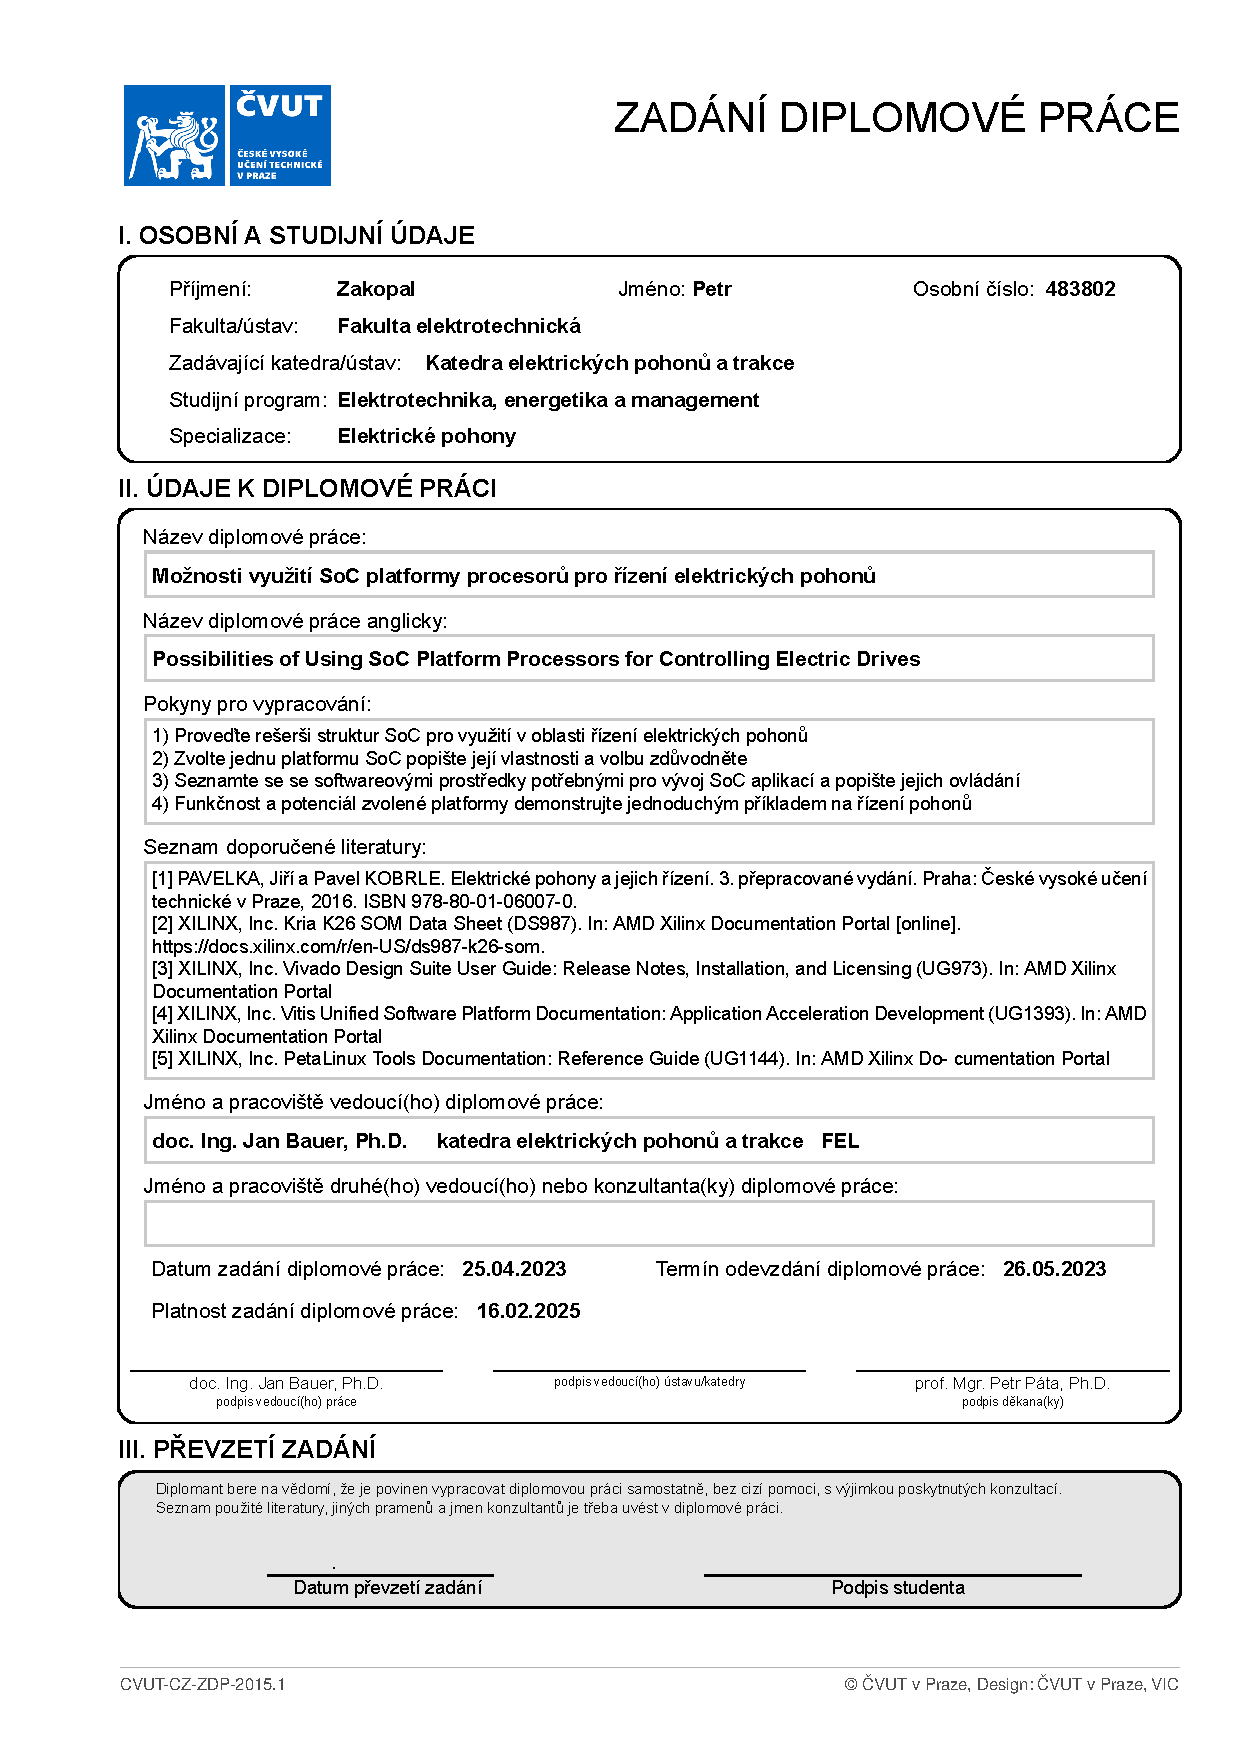
\includepdf[]{src/docs/zadani_bez_podpisu.pdf}

%\newpage
%\cleardoublepage
\null\newpage

\pagenumbering{Roman}
\setcounter{page}{5}%%3 NUTNO řešit dle zadání etc.

\noindent \textcolor{ctublue}{{\Large{\textbf{\MakeTextUppercase{Prohlášení}}}}}\\
			Prohlašuji, že jsem předloženou práci vypracoval samostatně a že jsem uvedl veškeré použité informační zdroje v~souladu s~Metodickým pokynem o~dodržování etických principů při přípravě vysokoškolských závěrečných prací.\\
		\vspace{1.5cm}
		
	

	\noindent	V~Praze dne \rule{3.5cm}{0.4pt} \hspace{6.6cm}  \rule{4cm}{0.4pt}
	
	\hspace{12.65cm}Petr Zakopal


		\vspace{14cm}
		
	\noindent	\textcolor{ctublue}{{\Large{\textbf{\MakeTextUppercase{Poděkování}}}}}\\
	Tímto bych rád poděkoval vedoucímu této práce doc. Ing. Janu Bauerovi, Ph.D. za skvělé vedení práce a cenné rady při vytváření. Dále bych rád poděkoval všem, kteří mě v~mých dosavadních studijních aktivitách podporovali.
		


%%ABSTRAKT%%

\newpage
%\addcontentsline{toc}{section}{3\quad Abstrakt a klíčová slova}%Added citations to TOC%
%\begin{comment}
\begin{minipage}[t]{7.37cm}
		%\raggedright
	\textcolor{ctublue}{\Large{\textbf{\MakeTextUppercase{Abstrakt}}}}\\
	Cílem této práce je realizovat pracoviště s~měničem DCM ovládaným pomocí PLC a představit relevantní teorii k~řešené problematice stejnosměrných cize buzených motorů, jejich řízení a základním schématům pro řízení těchto motorů pomocí usměrňovačů. Výsledky této práce popisují konfiguraci DCM měniče a vytvořený PLC a HMI program, potřebný pro ovládání pracoviště, a umožňují čtenáři získat základní teoretické vědomosti potřebné k~možnému přístupu na realizované pracoviště s~DCM.\\
	\textbf{Klíčová slova:} ČVUT FEL, katedra elektrických pohonů a trakce, stejnosměrný cize buzený motor, čtyřkvadrantový reverzační usměrňovač, pracoviště s~měničem DCM, PLC Siemens S-1200, HMI, zápis a čtení dat pomocí PLC, SINA\_PARA komunikace
\end{minipage}%
\hfill% --- important, otherwise it wont be so nice
\begin{minipage}[t]{7.37cm}
		\textcolor{ctublue}{\Large{\textbf{\MakeTextUppercase{Abstract}}}}\\
		The goal of this thesis is to explain basic theory of direct current separately excited motors and their control with rectifiers. It aims to introduce the reader to a PLC program controlling Siemens DCM drive. Ending purpose of this text is to explain how to control motor with a Siemens DCM rectifier in a conjuction with PLC and HMI programs. Reading this text may equip reader with fundamental knowledge which can be used at workplace with DCM drive. This text explains configuration of DCM drive and creation of PLC and HMI programs used for controlling the drive.\\
		\textbf{Keywords:} CTU FEE, Department of Electric Drives and Traction, direct current motor, four quadrant reverse rectifier, workplace with DCM Siemens Rectifier, PLC Siemens S-1200, HMI, reading and data writing via PLC, SINA\_PARA block communication
\end{minipage}
%\end{comment}
	%\textcolor{ctublue}{\Large{\textbf{\MakeTextUppercase{Abstrakt}}}}\\

	%\textcolor{ctublue}{\Large{\textbf{\MakeTextUppercase{Abstract}}}}\\

\newpage
\tableofcontents
\newpage%
\flushbottom %vyčištění stránky
\newpage
\vspace{0pt}
\listoffigures %seznam obrázků
\flushbottom %vyčištění stránky
\newpage
\listoftables
\flushbottom
\newpage


\pagenumbering{arabic} %to arabic page numbering - enabling page numbering after gobble which disabled page numbering
\pagenumbering{gobble}
\null\newpage
\null\newpage %PŘI VERZI ONLINE
\setcounter{page}{1}
\pagenumbering{arabic}
\fontspec{Times New Roman}

\section{Úvod}
V době, kdy byla od elektrických pohonů požadována spolehlivost, vysoká účinnost a nenáročné ovšem kvalitní řízení, byly k řízení využívány samotné digitální signálové procesory. Postupem času dochází ke zjištění, že výkon DSP není dostatečný a na některé aplikace, kde je vyžadováno provedení značné množství náročných výpočtů za co nejkratší čas, nejsou vhodné. Proto nastupuje éra logických programovatelných polí (FPGA), které jsou schopny tyto výpočty provést s velmi nízkými nároky na energii a za velmi krátký čas.\par
V mnoha odvětvích se již začíná využívat embedded systém s Application Spefified Hardware, který je určen pouze na využití v předem dané aplikaci. Tento hardware slouží v dané aplikaci k jedinému účelu, který vykonává a na který je optimalizován. Tím se liší od procesoru, který vykonává mnoho instrukcí a využít ho pouze jako samostatnou výpočetní jednotku je z hlediska energetické i finanční náročnosti nevýhodné. Implementace hradlových polí přináší nejen v řízení elektrických pohonů zvýšení výpočetního výkonu, ale také snižování energetické náročnosti řízení.\par
Perspektiva logických programovatelných polí a hardwaerově urychlovaných aplikací je podpořena jejich využíváním i mimo obor elektrických pohonů a trakce. Z důvodu jejich veliké propustnosti, vysokých výpočetních výkonů a nízké energetické náročnosti jsou využívány v AI, machine learningu, zpracování obrazu, těžení kryptoměn a jiných nepohonářských aplikacích.\par
Nevýhodou problematiky FPGA je jejich složitější programovatelnost z hlediska tvoření aplikace. Aplikace je tvořena určitým postupem (workflow), který kladne vysoké nároky na vzdělání a zkušenosti vývojářů. Většina FPGA je programována pomocí jazyků Verilog či VHDL, které mohou pro softwarově orientované programátory představovat značnou překážku. Proto bylo vyvinuto tvoření aplikací pomocí vyšší úrovně syntézy (HLS), kdy je možné tvořit programy ve vyšších programovacích jazycích jako je například C, C++ či Python. HLS umožnilo rapidní rozšíření a využití Embedded FPGA Accelerated Applications v mnoha aplikacích a značně vylepšilo vývojářský požitek (developer experience, DX) při tvorbě aplikací.\par
Protože může být náročné vytvořit vlastní architekturu, složenou z CPU a spolupracujícího FPGA, je vhodné při prvotním vývoji aplikace využít dostupné vývojové desky obsahující již předpřipravené propojení jednotlivých komponent. Součástí těchto vývojových desek bývá také mnoho vstupů a výstupů (I/O) pro snadnější využití při lazení a tvoření aplikace. V této práci je využívána vývojová deska Zybo od firmy Digilent. Ovšem autor v textu představuje další možnosti, které mohou být pro konkrétní aplikace a využití vhodnější.\par
Tato práce se zajímá o aplikace a možné využití FPGA při řízení elektrických pohonů. Autor v ní představuje základní principy Hardware Accelerated Applications, z jakého důvodu je tento přístup perspektivní a proč je vhodné se orientovat tímto směrem.\par
\flushbottom %vyčištění stránky
\newpage
%konec úvodu

\section{Teoretický základ}
	\subsection{Embedded Systems}
	Embedded systémy je název pro skupinu zařízení, obecně systémů, které je možné charakterizovat jako specifické výpočetní zařízení, resp. počítače, které jsou určeny pro podporu funkce nebo řízení nějakého většího celku či produktu. Oproti tomu osobní počítač je sice výpočetní zařízení, ale nelze mluvit o embedded systému, protože je určen pro mnoho univerzálních aplikací. \cite{Sass2010}\par
	Dalším důležitým rozdílem mezi \textit{Embedded System} a obecným výpočetním zařízením je ten, že v případě embedded systému je interakce mezi systémem a uživatelem uměle omezena na základní ovládání či kontrolu funkce. Není předpokládáno, že by uživatel, jež aplikaci embedded systému využvá, výrazným způsobem zasahoval do jeho funkce. Naopak obecný výpočetní systém je uzpůsoben na podstatné zásahy uživatele.\par
	Do embedded systému obecně vstupují vstupní signály, které jsou následně zpracovány a poté vybrané výsledky výpočtů jsou v podobě výstupní signálů výstupním produktem systému. Tyto signály většinou přicházejí ze speciálních snímačů, kompatibilních s embedded systémem (senzor teploty, senzor tlaku, senzor zrychlení, gyroskop apod.). Naopak jeho výstupem jsou přímo konektory, na kterých se dle požadavků objevuje např. specifická hodnota napětí. Nebo mohou na výstupních pinech výt připojené LED signalizace, komunikační sběrnice některých komunikačních systémů nebo výstupní LDC displaye. Způsob, kterým jsou kódovány vstupní a výstupní signály je většinou specificky určený aplikaci daného systému. \cite{Sass2010}\par
K obecnému výpočetnímu systému je možné připojit vstupní periferie klasických osbních počítačů – myš, klávesnice, mikrofon. Jako hlavní výstupní periferie obecného systému je monitor. Jeho komunikace s periferiemi je většinou standardizována tak, aby bylo možné periferie libovolně zaměňovat bez změny funkčnosti. \cite{Sass2010}.
		\subsubsection{Application Specific Integrated Circuit}
		S tématem embedded systémů se pojí pojem hardware, který je určen pro jedinou aplikaci. Tato skupina zařízení se nazývá \textit{Application Specific Integrated Circuit, popř. Hardware} (ASIC, ASHW). V této oblasti je opět využíváno přesvědčení, že pokud je architektura HW přímo specializovaná na jednu aplikaci, je vysoká pravděpodobnost, že ji bude vykonávat bezchybně, kvalitně a rychle.\par
		Tyto aplikace jsou využívaný v širokém spektru oborů jako je např. zpracování zvuku, videa, výpočtů apod. Tyto ASIC mohou také vykonávat potřebné rychlé výpočty pro matematické modely elektrických strojů, které jsou využívány např. pro HIL.\par
		Než je tento specifický obvod vytvořen, je nutné jej navrhnout, vyzkoušet a odladit. K tomu slouží logická programovatelná pole, ve kterých je možné požadovaný HW navrhnut a odladit před velko produkcí ASIC. Pokud velko produkce není z ekonomických důvodů možná, jsou FPGA využívány i v produkční oblasti, kde je HW struktura, která by byla přítomna na ASIC, vytvořena přímo na FPGA.
		\subsubsection{Hardware Accelerated Applications}
		V mnoha aplikacích, nejen při řízení elektrických pohonů, je vyžadováno, aby výpočty nebo zpracování dat probíhalo vysokou rychlostí. Tento problém nemůže být většinou vyřešen použitím běžného procesoru (CPU), který je optimalizován na provádění obecných komplexních funkcí řízení běhu programu, komunikace či přesunu dat. V moderním světě dochází k exponenciálnímu nárůstu množství dat, které je potřeba zpracovat. Aby tyto data bylo možné v požadovaném čase zpracovat, je třeba využít specifický HW, který bude schopen požadavky rychlosti a výkonu uspokojit. Tento proces se nazývá \textit{Hardware Acceleration}. \cite{xilinx-accelerated-computing}\par
		Princip hardwaerové akcelerace spočívá v přesunu výpočetně náročných aktivit na zvláštní oddělený hardware. Celkové řízení běhu aplikace a komunikace je ovšem stále přítomno na řídícím CPU. Oddělený hardware, na kterém dochází k akceleraci výpočtů je optimalizován na vykonávanou úlohu a jeho využití přináší zefektivnění běhu celkové aplikace. \cite{xilinx-accelerated-computing}\par
		Struktura, ve které je využíváno více oddělených hardwarových procesorových a akceleračních jednotek, se často nazývá heterogenní. \cite{xilinx-accelerated-computing}\par
		Hardwaerová akcelerace poskytuje rychlejší výpočty než CPU, protože využívá značné úrovně paralelismu výpočtů. Oproti tomu klasické CPU vykonává jednotlivé instrukce sériově. I v případě, že CPU má více jader a využívá více vláken, nemůže se úrovni paralelismu při dané energetické náročnosti HW vyrovnat.\par
		Pro HW akceleraci je v mnoha oblastech využíváno několik druhů jednotek, které jsou optimální pro dané aplikace.\par
		\textbf{Graphics Processing Units} (GPUs) jsou jednotky, které převážně slouží k akceleraci zpracování a renderování grafických úloh. V době rapidního rozvoje elektroniky a SW je možné využití GPUs v mnoha odvětví umělé inteligence (AI) či kreativních odvětích. GPUs jsou využívány v aplikacích, kde není kladen veliký důraz na nízkou odezvu (latenci). \cite{xilinx-accelerated-computing}\par
		\textbf{Tensor Processing Units} (TPUs) jsou jednotky, které slouží k provádění algoritmů strojového učení (machine-learning, ML). Jejich přímé datové propojení umožňuje velmi rychlý a přímý přenost dat. Díky přímému připojení nevyžadují využití pamětí, kter= by přenos dat zpomalovali. \cite{xilinx-accelerated-computing}\par
		\textbf{Field Programmable Gate Arrays} (FPGAs) jsou jednotky, ve kterých není při výrobě pevně daná HW struktura. To umožňuje vytvoření, resp. naprogramování HW dle požadavků akcelerované aplikace. FPGAs jsou využívány i v on-line výpočtech matematických modelů elektrických strojů. Při realizaci této práce je pro akceleraci využíváno právě těchto programovaelných polí.
	\subsection{Logické programovatelné pole – FPGA}
		\subsubsection{Popis funkce}
		\subsubsection{Programování}
		% VHDL vs HLS
		\subsection{Využití}
			\subsection{Spotřeba}
			\subsection{Výpočetní výkon a propustnost}
			\subsubsection{Aplikace v elektrtických pohonech}
			% HIL
			% Control
			% Control and Extended Kaufmann Filter
	\subsection{Vývojová deska Digilent Zybo}
		\subsubsection{Parametry a složení}
		% I/O
		% FPGA
		% CPU
		% RAM
		\subsubsection{Možné alternativy}
			% Novější verze Zybo
			% Něco jiného
			% Custom řešení - ZynQ Berry
			%  [ZynQBerry](https://shop.trenz-electronic.de/en/TE0726-03-11C64-A-ZynqBerry-Module-with-Xilinx-Z-7007S-Single-Core-Raspberry-Pi-2-compatible) (velice zajímavější i díky ceně, ale možná by hodně cool bylo celé si udělat sám sestavu)

\section{Matematický model stroje}
	\subsection{Představení stroje}
	\subsection{Odvození modelu}
	\subsection{Optimalizace modelu}

\section{Program pro FPGA a CPU}
	\subsection{Použité nástroje}
		\subsubsection{Xilinx Vivado}
		\subsubsection{Xilinx Vitis}
		\subsubsection{Petalinux}
		\subsubsection{Programovací prostředí – operační systém Linux}
		% Jaké verze jsou momentálně podporované
		% Co je třeba nainstalovat za balíčky před započetím instalace
		% Jaký je flow aby byla možná příprava systému
		% Proč zrovna linux Open Source
	\subsection{Tvorba HW architektury Xilinx Vivado}
	% Basic popsání, možná si zjistit do hloubky co vše znamená
    % WorkFlow
    % Zjistit jak dát vstupem tlačítka a jak výstupy jako výstupy

	\subsection{Tvorba Petalinux}
	\subsection{Tvorba SW pro CPU a FPGA}

\section{Představení pracoviště}
\section{Dosažené výsledky}


		
%závěr
\newpage
\addcontentsline{toc}{section}{\numberline{}Závěr} 
\section*{Závěr}
Aliquam dapibus leo velit, ultrices eleifend mi feugiat eget. Aliquam euismod facilisis turpis, nec lobortis libero aliquet sit amet. Aenean suscipit ante eget ipsum viverra hendrerit. Ut sed massa sed nisi tempus dapibus in eu enim. Nullam vitae odio laoreet, malesuada purus non, faucibus orci. Lorem ipsum dolor sit amet, consectetur adipiscing elit. Etiam eget odio quis enim laoreet imperdiet nec eu nunc. Maecenas ut consequat purus. Duis faucibus risus nec metus cursus placerat. Phasellus sapien justo, laoreet in pulvinar ut, maximus nec velit.\par
	

\flushbottom %vyčištění stránky

%konec závěru

\newpage
\printbibliography[title={{Literatura}}]	
\nocite{*}
\addcontentsline{toc}{section}{\numberline{}Literatura} %Added citations to TOC%
	\appendix
	\titleformat{\section}{\color{ctublue}\fontspec{Times New Roman}\fontsize{15}{15}\bfseries}{Příloha \thesection:}{2.1em}{}
	\begin{appendices}
	\section{Seznam symbolů a zkratek}
		\subsection{Seznam symbolů}
			\begin{description}
			\item $\vec{F}$ (N) \hspace*{\parindent} vektor síly
			
		\end{description}
	\subsection{Seznam zkratek}
		\begin{description}
			\item DCM \hspace*{\parindent} DC Master
			
		\end{description}
	\end{appendices}
\end{document}
